\documentclass[]{article}
\usepackage{amsmath}
\usepackage{amssymb}
\usepackage{graphicx}
%opening
\title{}
\author{}

\begin{document}

\maketitle

\begin{abstract}

\end{abstract}

\section*{Exercise 1: Spurious Regression}
\subsection*{1.0 Set-up and Definitions}
\begin{itemize} 
	\item time series are generated as standardized random walk processes:
		\begin{align*}
			x_t &= \phi x_{t-1} + u_{x,t}, x_0=0, u_{x,t}  \overset{iid}{\sim}\mathcal{N}(0,1)\\
			y_t &= \phi y_{t-1} + u_{y,t}, y_0=0, u_{y,t}  \overset{iid}{\sim}\mathcal{N}(0,1)\\
			\phi &\in \left\{0.8, 1\right\}
		\end{align*}
		A DGP with $\phi=0.8$ is referred to as \textbf{AR(1)} and a DGP with $\phi=1$ as \textbf{random walk} in the text.
	\item two regression models are defined:
		\begin{align*}
			y_t &= \beta_1 +\beta_2 x_t + v_t, &(\text{spurious regression})\\
			y_t &= \beta_1 + \beta_2 x_t + \beta_3 y_{t-1} + v_t, &(\text{valid regression})
		\end{align*}
		The \textbf{spurious regression} model should be expected to produce an insignificant estimate of $\beta_2$ and an $R^2$ near 0.
		The \textbf{valid regression} model reduces to the DGP for $y_t$ given $\beta_1=\beta_2=0$ and $\beta_3=1$.
	\item The combination of above DGPs and regression models yield 4 permutations for which the authors report how the rejection frequencies of $H0: \beta_2=0$ change with increasing sample size n.
	\begin{align*}
		LRM_1: y_{t} &= \beta_{1} +\beta_{2}x_{t} + v_{t}, &x_t, y_t: I(1), \phi=1\\
		LRM_2: y_{t} &= \beta_{1} +\beta_{2}x_{t} + v_{t}, &x_t, y_t: AR(1), \phi=0.8\\
		LRM_3: y_{t} &= \beta_{1} +\beta_{2}x_{t} + \beta_{3}y_{t-1} + v_{t}, &x_t, y_t: I(1), \phi=1\\
		LRM_4: y_{t} &= \beta_{1} +\beta_{2}x_{t} + \beta_{3}y_{t-1} + v_{t}, &x_t, y_t: AR(1), \phi=0.8
	\end{align*}	
	\item In each simulation the DGP produce timeseries of length T = 6, 12, 60, 120, 240, 360, 480.
	\item A total of $N_{sim} = 100,000$ is run to produce the distributions of t-stat and $R^2$.
	\item Each regression model is estimated with OLS under asymptotic theory\footnote{ref: class notes, Ch 2, p. 60}
	\subitem \textbf{A.1: independent observations} $y_i, x_i$ are i.i.d, which is equivalent to $v_t|x$ and $v_t|y$ being i.i.d.
	\subitem \textbf{A.2: regressors are uncorrelated with errors} $E[v_t x_t]=E[v_t y_t]=0$. This assumption is weaker than strict exogeneity and is not restricting the utilization of lagged values of the dependent variable into the regressors matrix.
	\subitem \textbf{A.3 Identification} $Q= E[x_{t}x_{t}']$ exists, is positive definite and has rank corresponding to the total number of regressors (no regressor is a linear combination of the others).
	\subitem \textbf{A.4: Finite Moments } $S = E[v_{t}^2x_{t}x_{t}']$ exists and is positive definite, with 
		\begin{align*}
			S &= E[v_{t}^2x_{t}x_{t}']\\
			&= E[v_t^2]E[x_tx_t']+cov(v_t,x_t)\\
			&= E[v_t^2]E[Q], by A.2
		\end{align*}
\end{itemize}

\subsection*{1.a}
\subsubsection*{(i) Compute for each sample size T the distribution of the $R^2$ of the MC simulations with either 7 separate histograms, or one unique figure where you report on the y-axis the 5\%, 10\% 25\%, 50\%, 75\%, 90\% and 95\% quantiles of the distributions of the simulated $R^2$, and on the x-axis you have T = 6, 12, 60, 120, 240, 360, 480.}



\begin{figure}
	\centering
	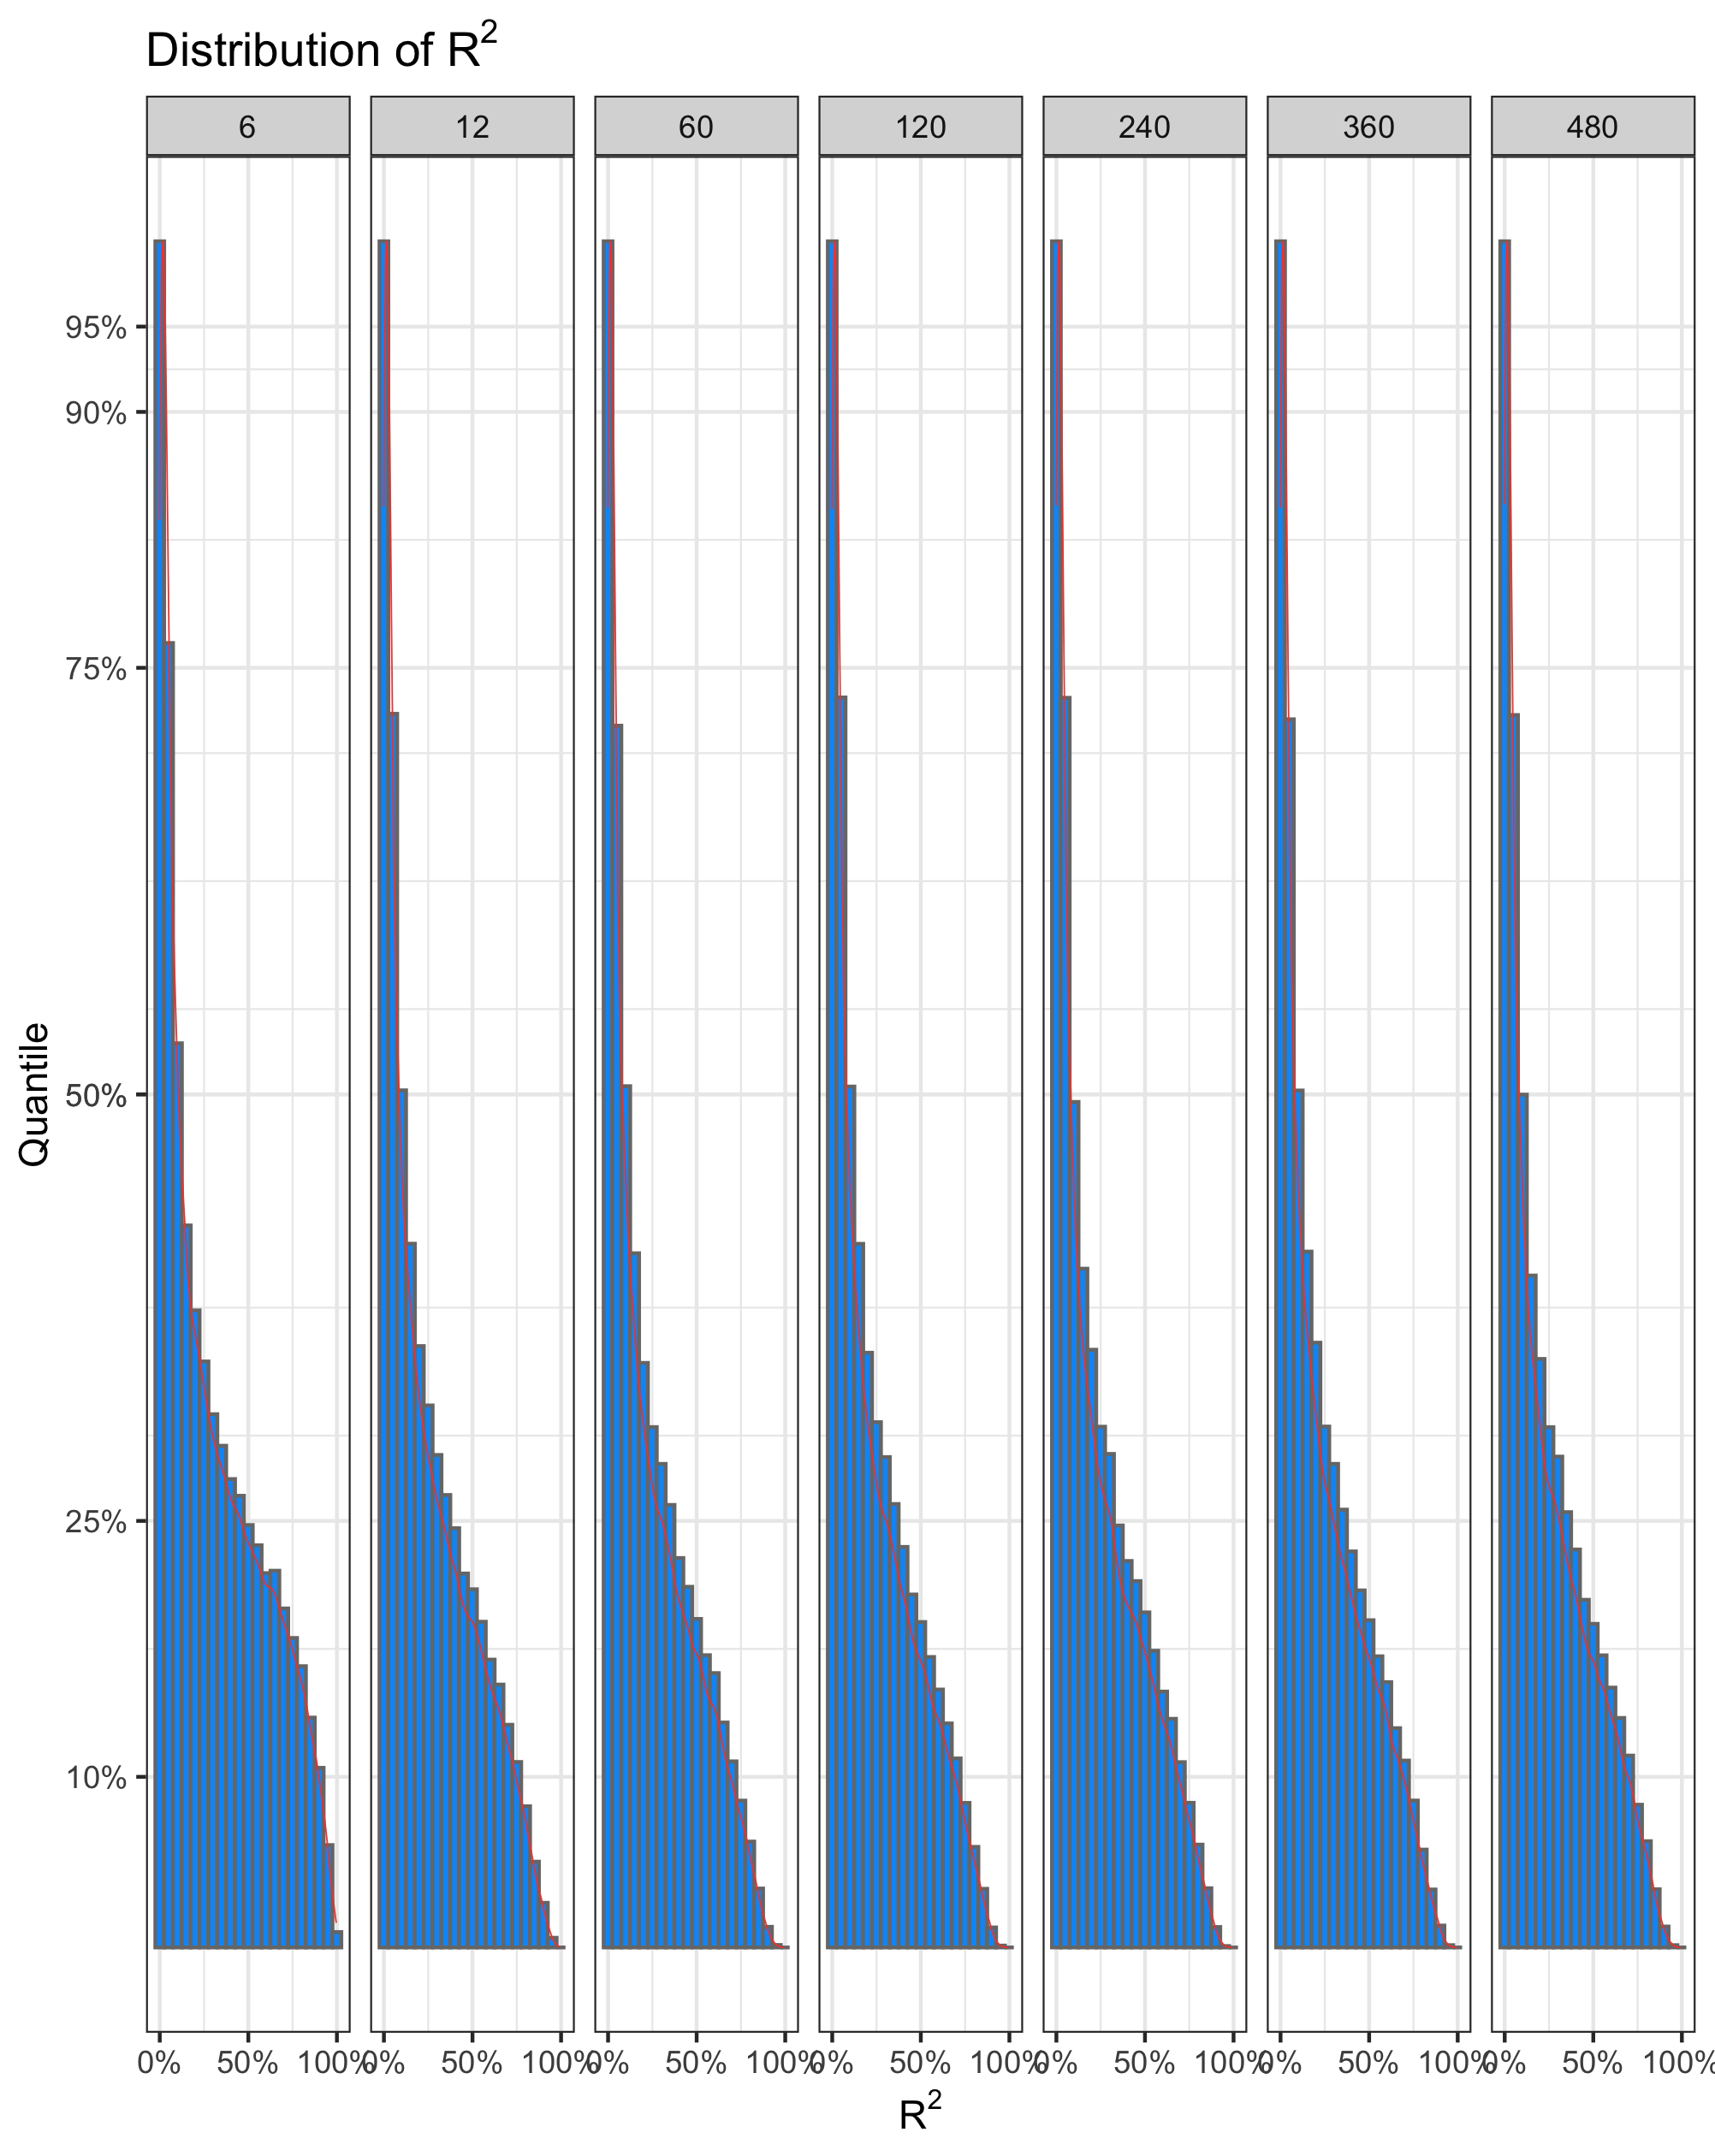
\includegraphics[width=0.7\linewidth]{"./1ai_chart.png"}
	\caption{}
	\label{fig:1aichart}
\end{figure}


\end{document}
